\documentclass[12pt]{report}

\newcommand{\titletext}{Spectraalanalyse Variabiliteit voor niet-lineaire systemen.}

\usepackage[dutch]{babel}
\usepackage[nobottomtitles]{titlesec}
\usepackage[bottom]{footmisc}
\usepackage{graphicx}
\usepackage{titleps}
\usepackage{amssymb}
\usepackage{amsmath}
\usepackage{amsthm}
\usepackage{graphicx}
\usepackage{verbatim}
\usepackage{titling}
\usepackage[toc,page]{appendix}
\usepackage{bm}
\usepackage{wrapfig}
\usepackage{subcaption}
\usepackage{algorithm}
\usepackage{algpseudocode}
\usepackage{algorithmicx}
\floatname{algorithm}{Algoritme}

\usepackage{fancyhdr}

\pagestyle{fancy}

\renewcommand{\chaptermark}[1]{\markboth{#1}{}}
\renewcommand{\sectionmark}[1]{\markright{#1}}
\fancyhf{}
\fancypagestyle{plain}{%
  \fancyhf{}%
    \rfoot{\fancyplain{}{\nouppercase{\thepage}}}
    \lfoot{\fancyplain{}{\nouppercase{\leftmark}}}
  \renewcommand{\headrulewidth}{0pt}% Line at the header invisible
  \renewcommand{\footrulewidth}{0.4pt}% Line at the footer visible
}
\lhead{\fancyplain{}{\titletext}}
\rhead{\fancyplain{}{Thorvald Dox}}
\rfoot{\fancyplain{}{\nouppercase{\thepage}}}
\lfoot{\fancyplain{}{\nouppercase{\leftmark}}}
\renewcommand{\footrulewidth}{0.4pt}

\fancyhfoffset[E,O]{0pt}
\date{}
  
\usepackage[margin=1in]{geometry}
\usepackage{float}



\usepackage[super,square,sort]{natbib}
\usepackage{bibentry}
\nobibliography*

%\newcommand{\footcite}[1]{\cite{#1}\let\thefootnote\relax \footnote{\cite{#1} \bibentry{#1}} }
\def\signed #1{{\leavevmode\unskip\nobreak\hfil\penalty50\hskip2em
  \hbox{}\nobreak\hfil(#1)%
  \parfillskip=0pt \finalhyphendemerits=0 \endgraf}}
\newcommand{\rulesep}{\unskip\ \vrule height -1ex\ }
\newcommand{\proj}[2]{\text{proj}_{#2}\left(#1\right)}

\DeclareMathOperator*{\Odot}{\bigodot}
\allowdisplaybreaks

%\title{Semi-lineair Multiple Endmember mixture spectrum analysis}
\title{\titletext}
\author{Thorvald Dox}

\begin{document}
\begin{titlepage}

\newcommand{\HRule}{\rule{\linewidth}{0.5mm}} % Defines a new command for the horizontal lines, change thickness here

\center % Center everything on the page
 
%----------------------------------------------------------------------------------------
%	HEADING SECTIONS
%----------------------------------------------------------------------------------------

\textsc{\LARGE Universiteit Antwerpen}\\[1.5cm] % Name of your university/college
\textsc{\Large Fysica}\\[0.5cm] % Major heading such as course name
\textsc{\large Masterproef}\\[0.5cm] % Minor heading such as course title

%----------------------------------------------------------------------------------------
%	TITLE SECTION
%----------------------------------------------------------------------------------------

\HRule \\[0.4cm]
{ \Large \bfseries \thetitle}\\[0.4cm] % Title of your document
\HRule \\[1.5cm]
 
%----------------------------------------------------------------------------------------
%	AUTHOR SECTION
%----------------------------------------------------------------------------------------

\begin{minipage}{0.4\textwidth}
\begin{flushleft} \large
\emph{Auteur:}\\
\theauthor % Your name
~\\
~\\
~\\
\end{flushleft}
\end{minipage}
~
\begin{minipage}{0.4\textwidth}
\begin{flushright} \large
\emph{Promotor:} \\
Paul {Scheunders} \\ % Supervisor's Name
\emph{Copromotor:} \\
Rob {Heylen} % Supervisor's Name
\end{flushright}
\end{minipage}\\[5cm]

% If you don't want a supervisor, uncomment the two lines below and remove the section above
%\Large \emph{Author:}\\
%John \textsc{Smith}\\[3cm] % Your name

%----------------------------------------------------------------------------------------
%	DATE SECTION
%----------------------------------------------------------------------------------------

%{\large \today}\\[3cm] % Date, change the \today to a set date if you want to be precise

%----------------------------------------------------------------------------------------
%	LOGO SECTION
%----------------------------------------------------------------------------------------

%
\includegraphics[height=4cm]{remote.png}

\includegraphics[height=4cm]{download.jpg}
\hspace{5 cm}

\includegraphics[height=4cm]{vlabsym.png}
 \\[1cm] % Include a department/university logo - this will require the graphicx package

 
%----------------------------------------------------------------------------------------

\vfill % Fill the rest of the page with whitespace

\end{titlepage}
\tableofcontents


\newpage
\chapter*{Abstract}
\addcontentsline{toc}{chapter}{Abstract (english)}


\newpage
\chapter*{Abstract}
\addcontentsline{toc}{chapter}{Abstract (Nederlands)}



\newpage
\chapter*{Structuur van deze thesis}
\addcontentsline{toc}{chapter}{Structuur van deze thesis}
 In de inleiding worden de fundamenten van aardobservatie beschreven.Dit hoofdstuk is vooral gebaseerd op 
\textit{Fundamentals of remote sensing\cite{fun}}.

Het eerste hoofdstuk introduceert het onderwerp van deze thesis: spectrale ontmenging. Eerst wordt het lineaire spectrale ontmengingsmodel beschreven, welke het meest gebruikte model is. Dan worden twee belangrijke problemen beschreven die niet met het lineaire model kunnen worden behandeld: niet-lineaire effecten en endmember variabiliteit.

In hoofdstuk 2 worden 2 state-of-the-art methodes uit de literatuur beschreven voor niet-lineair spectrale ontmenging en endmember variabiliteit.  Het multilineair model is een methode voor niet-lineaire spectrale ontmenging, en wordt uitvoerig beschreven in: \textit{A multilinear mixing model for nonlinear spectral unmixing}\cite{mlinmix}. De tweede methode brengt  endmember variabiliteit in rekening en wordt behandeld in: \textit{Hyperspectral unmixing with endmember variability via alternating angle minimization}\cite{mesma}.

Er zijn in de literatuur momenteel nauwelijks of geen methoden gekend die endmember variabiliteit in rekening brengen bij niet-lineaire ontmenging. Daarom heb ik in deze masterproef onderzoek gedaan naar de combinatie van niet-lineaire ontmenging en endmember variabiliteit. In het derde hoofdstuk beschrijf ik een aantal methodes die gelijktijdig rekening houden met beide concepten. Deze methodes zijn gebaseerd op combinaties van de 2 methodes uit hoofdstuk 2.
	
In hoofdstuk 4 worden de ontwikkelde methodes en een aantal varianten hierop gevalideerd  op een experimentele dataset: de Alina dataset\cite{Alina}.  
\newpage
\chapter*{Inleiding}
\addcontentsline{toc}{chapter}{Inleiding}

\begin{quotation}
Aardobservatie is de wetenschap van het bepalen van informatie over het aardoppervlak vanop een afstand. Dit wordt gedaan door het meten en vastleggen van gereflecteerde of uitgezonden electromagnetische golven en het verwerken, analyseren en toepassen van deze informatie.
\signed{\textit{Fundamentals of remote sensing\cite{fun} p5}}
\end{quotation}

\begin{wrapfigure}{R}{0.4\textwidth}
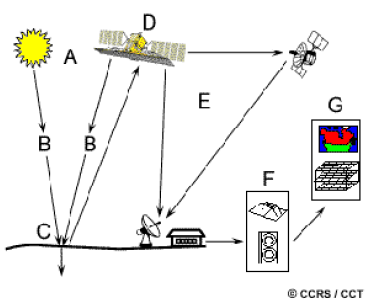
\includegraphics[width=0.4\textwidth]{rs.PNG}
\caption{Aardopservatie \label{fig:rs} Deze afbeelding komt uit \textit{Fundamentals of remote sensing\cite{fun}}}
\end{wrapfigure}


%Het gedetai\"eerde proces verloopt zoals hierna beschreven\cite{fun}, en is te zien in figuur \ref{fig:rs} .

%Een lichtstraal ontstaat aan een zo genaamde lichtbron, wat in de meeste gevallen de zon is. Deze lichtstraal reist door de ruimte en door de atmosfeer, tot deze contact maakt men een materiaal, en hierop een of meerdere keren reflecteert. Daarna reist deze lichtstraal opnieuw door de atmosfeer tot deze contact maakt met een camera op een satelliet. De eigenschappen van deze lichtstraal worden be\"invloed door elk van deze processen.

Aardobservatie begint bij een lichtbron\footnote{In het geval dat men ge\"interesseerd is in het thermisch infrarood spectrum, is er geen lichtbron nodig aangezien materialen op kamertemperatuur van nature dit soort licht uitstralen, ten gevolge van black body radiation.}. Dit is vaak de zon, maar dit proces is gelijkaardig voor andere lichtbronnen. De lichtbron zendt een lichtstraal uit, die eerst door de ruimte en vervolgens door de atmosfeer reist, totdat deze contact maakt met een materiaal op het aardoppervlak en hierop een of meermaals reflecteert. Deze reflectie verandert de eigenschappen van de lichtstraal. De gereflecteerde lichtstraal reist opnieuw door de ruimte, totdat deze in contact komt met de detector op een satelliet. Deze detector zet de lichtstraal om in elektrische signalen, die verzonden worden vanaf de satelliet naar het aardoppervlak, waar deze geanalyseerd kunnen worden. Dit volledige proces wordt afgebeeld op figuur \ref{fig:rs}. 



%Elke lichtstraal is een golf in het elektromagnetische spectrum. Deze golf wordt enerzijds bepaald door zijn golflengte, wat de lengte is tussen twee opeenvolgende maxima van de golf, zoals afgebeeld in figuur \ref{fig:golflengte}. Anderzijds wordt de golf bepaald door de intensiteit, wat de grootte is van de piek van de golf. Soms wordt de frequentie van de golf gebruikt om deze te karakteriseren, maar die kan bepaald worden uit de golflengte en de snelheid van het licht. In werkelijkheid is een lichtstraal niet een golf, maar een combinatie van verschillende golven met elk hun golflengte en intensiteit. De bijbehorende intensiteit bij elke golflengte wordt het spectrum genoemd.

\subsubsection{Elektromagnetische golven}
Een lichtstraal is een elektromagnetische golf, met als een van de belangrijkste eigenschappen voor aardobservatie de golflengte. Voor een vlakke golf is deze golflengte de afstand tussen twee opeenvolgende cycli, zoals te zien in figuur \ref{fig:rs2}. Echter, een lichtstraal is bijna nooit een vlakke golf, maar een combinatie van verschillende vlakke golven met verschillende golflengten. De intensiteit van elke vlakke golf op elke specifieke golflengte wordt het spectrum genoemd. Soms wordt in plaats van golflengte ook frequentie gebruikt, deze is eigenlijk de snelheid van het licht gedeeld door de golflengte.

\subsubsection{Hyperspectrale camera's}
Gewone beelden van een camera bestaan uit drie kleuren, elk passende bij een specifieke golflengte. De keuze voor deze drie kleuren, namelijk rood, groen en blauw, is een gevolg van de beperkingen van het menselijk oog. Het zijn de kleuren die een mens kan waarnemen. Om dit beeld digitaal te vertalen, moet het beeld opgedeeld worden in kleine, even grote, vierkante elementen, genaamd pixels. Elk van deze pixels bevat voor elke kleur een waarde, die de respectievelijke intensiteit van alle kleuren in dit vierkant weergeeft. Hyperspectrale camera's werken in essentie op dezelfde manier, alleen detecteert deze camera niet alleen de hoeveelheid rood, groen en blauw, maar een groot aantal kleuren, genaamd banden. Door het grotere aantal banden in vergelijking met die van een gewone camera, kan hier meer informatie uit gehaald worden. De zon zendt vooral licht uit in het infrarood, het zichtbaar licht en het ultraviolet en daarom worden er vooral banden gebruikt uit dit spectrum, zoals te zien in figuur \ref{fig:specs}.


\begin{figure}
\center
\begin{subfigure}[b]{0.3\textwidth}
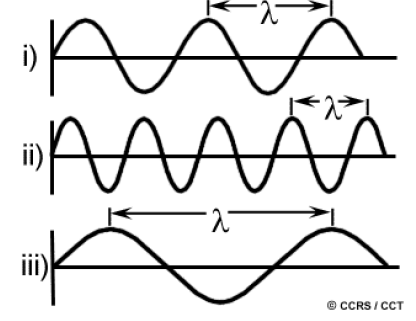
\includegraphics[width=\textwidth]{golflengte.PNG}
\caption{Golven met verschillende golflengten \label{fig:golflengte}}
\end{subfigure} \rulesep
\begin{subfigure}[b]{0.2\textwidth}
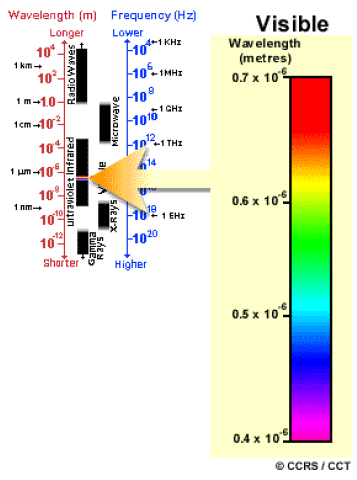
\includegraphics[width=\textwidth]{spec.PNG}
\caption{Het electromagnetische spectrum. \label{fig:spec}}
\end{subfigure}\rulesep
\begin{subfigure}[b]{0.4\textwidth}
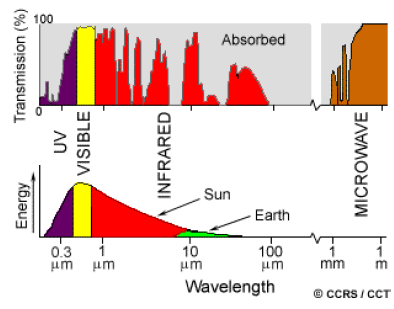
\includegraphics[width=\textwidth]{spec2.PNG}
\caption{Het spectrum van de zon. \label{fig:specs}}
\end{subfigure}
\caption{Electromagnetische golven. Deze afbeeldingen komen uit \textit{Fundamentals of remote sensing\cite{fun}}\label{fig:rs2}}
\end{figure}


Het doel van spectrale analyse is het bepalen van de hoeveelheden van elk materiaal op het aardoppervlak in een specifieke pixel, gegeven het spectrum van deze pixel. Verschillende methoden hiervoor worden beschreven in deze thesis. 

\section{Reflectie} \label{sec:ref}

%Wanneer een lichtstraal invalt op een materiaal reflecteert deze een gedeelte van dit licht. Het nieuwe spectrum van het gereflecteerde licht kan bepaald worden aan de hand van de eigenschappen van het materiaal en het spectrum van het binnenkomende licht. Er kan de benadering gemaakt worden dat de intensiteit voor een gegeven frequentie van het gereflecteerde spectrum alleen afhankelijk is van de intensiteit van het invallende spectrum, en deze daar recht evenredig aan is. In dit geval kan de reflectie beschreven worden als een Hadamard van het spectrum van de inkomende straal en het ``spectrum'' van het materiaal. Dit spectrum is nu geen vector van intensiteiten weer, maar een vector die voor elke frequentie bevat welk deel van de inkomende lichtstraal wordt gereflecteerd. 

Wanneer een lichtstraal invalt op een materiaal reflecteert dit een gedeelte van het licht en absorbeert het de rest. Het spectrum van deze lichtstraal die gereflecteerd wordt noemt men de reflectantie. Deze is afhankelijk van het materiaal en van de golflengte van het licht. 

In deze thesis worden hiervoor drie aannames gemaakt. Ten eerste: de gereflecteerde lichtstraal heeft dezelfde golflengte als het invallende licht. Ten tweede: de intensiteit is van de gereflecteerde straal recht evenredig met de intensiteit van de invallende straal. Ten derde: de reflectie van een lichtstraal van een specifieke golflengte wordt niet be\"invloed door licht van andere frequenties. Deze drie aannames zijn correct in de klassieke fysica, maar er zitten correcties van kwantummechanische effecten op. Deze zijn echter klein genoeg zodat ze als deel van de ruis beschouwd kunnen worden.

De intensiteit van de uitgaande straal kan geschreven worden als volgt:

\begin{equation}
E_{out}(\lambda) = R_\lambda E_{in}(\lambda)
\end{equation}

Dit is een stelsel van vergelijkingen met een vergelijking voor elke waarde van $\lambda$, die overeenkomt met een band in het spectrum. Zowel de intensiteiten als de reflectieco\"efficienten kunnen samengesteld worden tot een vector, en dan geldt

\begin{equation}
\bm{x} = \bm{R}\odot \bm{y}
\end{equation}

met $\odot$ het Hadamard ofwel elementwijs product. De vector $R$ is de reflectie van het materiaal. Deze neemt in beschouwing dat er meerdere interacties kunnen gebeuren in het materiaal. Een reflectie die alleen een enkelvoudige interactie meeneemt, noemt men het albedo.


\section{Atmosferische correctie}

Wanneer de lichtbron uniform en genormaliseerd is, is de reflectie gelijk aan de reflectantie. Alleen is de gebruikte lichtbron - meestal is dit de zon - niet uniform. Verder be\"invloeden verschillende effecten de lichtstraal\cite{fun} zoals verschuiving, atmosferische verstrooiing, Rayleigh verstrooiing, Mie verstrooiing, nonselectieve verstrooiing, atmosferische absorptie, ozon absorptie, $CO_2$-absorptie en interpixel verstrooiing. De gebruikte datasets in deze thesis zijn door een algoritme gecorrigeerd voor al deze effecten, en de beelden kunnen dus beschouwd worden als verlicht door een uniforme lichtbron, waarbij de gedetecteerde lichtstraal alleen be\"invloed is door reflecties en Gaussische ruis. 

\section{Toepassingen}

Een veelgebruikte toepassing van aardobservatie is het in kaart brengen van landbouwgewassen\cite{fun}. Men kan niet alleen het soort gewas op een akker in kaart brengen, maar ook de gezondheid en verwachte oogst van verschillende gewassen. In het verleden werd het in kaart brengen van gewassen gedaan door steekproeven met de hand vanop de grond te nemen, maar aardobservatie is nauwkeuriger, goedkoper en kan gestandaardiseerd worden. Enerzijds is deze informatie nuttig voor de landbouwers zelf, omdat deze aan de hand van de data kunnen bepalen welke gewassen het beste groeien op welke plaats en wanneer er het best gezaaid of geoogst wordt, aan de andere kant is deze informatie ook nuttig voor overheden en verzekeraars, omdat deze kunnen nagaan welke planten er geplant worden, voorspellen wat de oogst gaat zijn en de schade  bepalen na een droogte of storm. 

Aardobservatie wordt ook toepast in de geologie. Van de aardbodem kan niet alleen het soort gesteente aan de oppervlakte in kaart gebracht worden, maar ook de formatie van deze gesteentes en zelfs de gesteentes liggend onder de aardbodem. Een van de voor de hand liggende toepassingen hiervan is de mijnbouw; een andere, het voorspellen van aardbevingen, aardverschuivingen en vulkanisme, wat inhoudt dat aardobservatie gebruikt kan worden voor het plannen van wegen, gebouwen en andere structuren. 

  
\begin{figure}
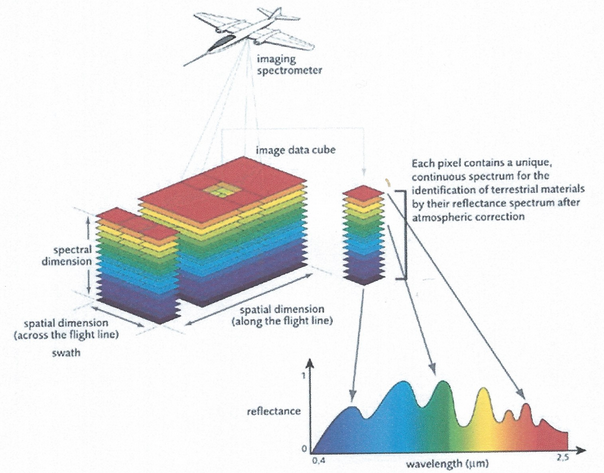
\includegraphics[width=\textwidth]{hyp.PNG}
\caption{Opbouw van een hyperspectraal beeld. Deze afbeelding komt uit \textit{Fundamentals of remote sensing\cite{fun}}}
\end{figure}

\chapter{Spectraal ontmengen}



%Het doel van spectrale anaylise is om uit deze hyperspectrale beelden het bepalen welke materialen zich op een specifieke pixel bevinden. Hoewel het belangrijkste toepassing hiervan de aardopservatie is, kan dit evidenterwijs ook gebruikt worden om materialen te analyseren in een laboratorium of voor bijvoorbeeld kwaliteitscontrole in de industrie.

\section{Resolutie}

Een pixel in een hyperspectraal beeld bevat een of meerdere materialen. Indien elke pixel maar een enkel materiaal zou bevatten, zou elk spectrum van elke pixel vergeleken kunnen worden met een referentiespectrum. Echter, het is theoretisch onmogelijk om een camera te maken met een resolutie die groot genoeg is om dit te verwezenlijken. De hoeveelheid licht die op de camera valt is immers beperkt, en moet verdeeld worden over alle pixels en de verschillende banden. Dit betekent dat wanneer de pixels te klein worden, elke pixel te weinig licht krijgt en de signaal-ruisverhouding te laag wordt, en aangezien licht bestaat uit fotonen, is er een limiet aan de gevoeligheid van de camera. 

De enige methode om de gevoeligheid te verhogen is bijgevolg een langere belichtingstijd. Hierdoor vergroot de ruis en dit is niet haalbaar voor een satelliet in een baan rond de aarde - zelfs als het praktisch haalbaar is om de resolutie kleiner te maken, ligt het probleem vooral in de fractalische eigenschappen van vele objecten. 

Als bijvoorbeeld, bij het observeren van een bos een grove resolutie gebruikt wordt, vallen er verschillende soorten bomen in een enkele pixel. Als de pixels kleiner worden, kunnen bomen al van elkaar onderscheiden worden, maar de takken van die bomen nog niet. Zelfs een blad bestaat nog uit verschillende materialen, aangezien de nerven van het blad uit een ander materiaal bestaan dan de bladmoes. Ook bij mineralen heeft men eenzelfde probleem: een gesteente bevat verschillende mineralen, maar om deze van elkaar te kunnen onderscheiden moet de pixelgrootte van microscopisch niveau zijn. 

Hierom is het van belang om het spectrum van een pixel, dat een combinatie is van de spectra van de verschillende materialen in deze pixel, te kunnen ``ontmengen''. Hierbij is men specifiek ge\"interesseerd in de abundantie van elk materiaal: een getal dat het gedeelte van de lichtstralen afkomstig van dat specifiek materiaal in een pixel weergeeft. Aangezien dit een goede maat is voor de aanwezige hoeveelheid van een bepaald materiaal in een pixel, is dit de belangrijkste parameter.

\section{Spectrale analyse}

Het spectrum van licht kan beschreven worden als een wiskundige functie die frequentie omzet in intensiteit. een hyperspectraal beeld bevat niet de volledige functie, maar bevat tweehonderd waarden uit deze functie, de zogenoemde banden. In matlab\citep{MATLAB} wordt dit opgeslagen als een driedimensionale tensor, waarbij de verschillende assen de $x$ positie, $y$ positie en de band van de pixel weergeven. 

In deze thesis is men niet ge\"interesseerd in interpixel-interacties, er wordt vanuit gegaan dat het materiaal in een pixel geen invloed heeft op het spectrum van andere pixels. Correcter zegt dit dat de materialen in een enkele pixel niet meer invloed hebben op naastliggende pixels dan op andere willekeurige pixels in het beeld. Daardoor is de exacte structuur van de pixels niet van belang en kan deze worden vervangen door een lijst van pixels die elk afzonderlijk ontmengd moeten worden.  Hierdoor kan de drie-dimensionale tensor worden omgezet in een matrix, waarin de rijen de verschillende pixels zijn en de kolommen de banden.  


%\begin{itemize}
%\item spectra als functies (eigenschappen van licht)
%\item spectra als vector (endmembers) $\rightarrow$ matlab implementatie
%\item mengen van endmembers (abundancies)
%\end{itemize}




\section{Lineair ontmengen}

Bij lineair ontmengen wordt uitgegaan van het \textit{linear mixing model}. Een lichtstraal valt in op een pixel op een enkel wel bepaald materiaal, interageert eenmalig met dit materiaal en valt daarna op de detector. Het spectrum van de teruggekaatste lichtstraal alleen afhangt van de reflectantie van het materiaal, de \textit{endmember} genaamd. De totale reflectantie van een gemeten pixel is het gewogen gemiddelde van de verschillende endmembers, waarbij het gewicht van elke endmember bepaald wordt door het gedeelte van de lichtstralen dat door dit materiaal gereflecteerd wordt. Dit gedeelte is de abundantie. In symbolen geeft dit:


% waarbij uitgegaan wordt dat elke lichtstraal die op een pixel valt enkelvoudig reflecteert en daarna op de detector valt. Het totale spectra op de detector is het gewogen gemiddelde van de spectra van de verschillende endmembers, waarbij het gewicht voor elke endmember de abundantie is van deze endmember. Men krijgt volgende uitdrukking: 


\begin{align}
\bm{x} &= \sum_i a_i \bm{e}_i \label{eq:nq}
\end{align}

Waarbij $\bm{x}$ het gemeten spectrum is, $e_i$ de endmembers en $a_i$ de abundanties. Omdat het mixing model slechts een benadering is van de werkelijkheid en omdat er op een experimentele meting altijd een vorm van ruis zit, kan het exacte spectrum nooit gevonden worden. Er wordt daarom gezocht naar het reconstructiespectrum dat het dichtst bij het werkelijke spectrum ligt. Hierbij wordt verondersteld dat de ruis normaal verdeeld is. Dit is een eenvoudig gevolg van het centrale-limiettheorema, dat zegt dat de som van een groot aantal kansvariabelen normaal verdeeld is. 

Noem $\bm{x}$ het gemeten spectrum, en $\bm{y}$ het reconstructiespectrum, met $\bm{\eta}$ de ruis, dan is

\begin{equation}\label{eq:rec0}
\bm{x} = \bm{y} + \bm{\eta}
\end{equation}

De kans dat $\bm{x}$ gemeten wordt, gegeven dat $\bm{y}$ het reconstructiespectrum is, is $f(\eta)$, waarbij $f$ de normale verdeling is. Aangezien de normale verdeling afhankelijk is van de kwadratische norm, zijn we alleen ge\"intereseerd in de kwadratische norm van de ruis. De normale verdeling is ook groter wanneer deze kwadratische norm kleiner is, dus moet de norm van de ruis geminimaliseerd worden om de kans te maximaliseren.  

Deze norm kan berekend worden gebruik makend van vergelijking \ref{eq:rec0}.

\begin{eqnarray}
\left|\bm{\eta}\right| &= \left|\bm{x} - \bm{y}\right| \label{eq:rec}
\end{eqnarray}

De uitdrukking $\left|\bm{x} - \bm{y}\right|$ noemt men het reconstructie-error. Het is deze uitdrukking die geminimaliseerd moet worden bij ontmenging. 


\subsection{Minimaliseren van reconstructie-error}
Voor het lineair model wordt er vanuit gegaan dat de endmembers gekend zijn, maar de abundanties en de ruis niet. Als de ruis wordt toegevoegd aan vergelijking \ref{eq:nq} dan geldt:

\begin{align}
\bm{x} &= \sum_i a_i \bm{e}_i + \eta
\end{align}

Het minimaliseren van de reconstructie-error, gebruik makend van vergelijking \ref{eq:rec}:

\begin{align}
\text{argmin}_{a_1 ... a_p} \left| \bm{x} - \sum_{i=1}^p a_i \bm{e}_i\right|^2
\end{align}

Indien de abundanties $a_i$ vrije re\"ele waarden zouden zijn, zou dit minimum eenvoudig berekend kunnen worden, door een projectie te nemen opgespannen door het vlak van de endmembers. Deze projectie kan genomen worden als volgt. Neem $E = [e_1,e_2,...,e_n]$ een matrix met als kolommen de verschillende endmembers. De projectie op de deelruimte opgespannen door de elementen van $E$ kan gevonden worden aan de hand van de \textit{Penrose-inverse} matrix.

\begin{equation}
\bm{a} = (E^T E)^{-1} E^T \bm{x}
\end{equation}

Doordat de abundanties gedeeltes van lichtstralen zijn die op een materiaal botsen, zijn er twee extra voorwaarden. Enerzijds moeten de abundanties positief zijn, aangezien men geen negatieve hoeveelheid lichtstralen kan hebben - dit noemt men de niet-negativiteitsvoorwaarde; anderzijds kan elke lichtstraal maar op een enkel materiaal botsen, dus is de som van alle gedeeltes \'e\'en - dit noemt men de eenheidssom-voorwaarde.  


\subsubsection{Niet-negativiteit}

De niet-negativiteitsvoorwaarde geeft weer dat de abundanties allemaal positief moeten zijn, dus groter dan nul. Dit betekent dat men niet moet projecteren op de deelruimte, maar op een deelverzameling ervan. Hiervoor kan een aangepast algoritme gebruikt worden, namelijk het ``nonnegative least-squares curve fitting'' of \texttt{lsqnonneg} algoritme. Dit algoritme is veel berekeningsintensiever dan het \textit{penrose-inverse} algoritme. Later in sectie \ref{sec:select} wordt een alternatieve methode beschreven om met deze voorwaarde om te gaan.

\subsubsection{Eenheidssom}

De eenheidssom-voorwaarde geeft weer dat de abundanties moeten sommeren tot \'e\'en. Dit zorgt ervoor dat de mogelijke abundanties geen deelruimte meer opspannen, aangezien het nulpunt geen element meer is van het hypervlak. Dit kan worden opgelost door een van de endmembers als schaduw te beschouwen. Dit verschuift het hypervlak over de vector $e_1$ zodanig dat het nulpunt deel wordt van de hyperruimte en dit terug een deelruimte is.

Deze transformatie houdt in dat de matrix $E$ getranslateerd wordt naar $[e_2-e_1;e_3-e_1;...;e_n-e_1]$ en het gemeten spectrum naar $\bm{x} - e_1$. Na deze transformatie kan het \textit{Penrose-inverse} algoritme worden toegepast, zodat men de abundanties $a_2,a_3,...,a_n$ krijgt. De laatste abundantie $a_1$ kan gevonden worden door de eenheidssomvoorwaarde te eisen, zodat $a_1 = 1 - \sum{i=2}^{n} a_i$.

\vspace{5 mm}
Het algoritme dat beide bovenstaande correcties doorvoert is het \textit{Fully constrained
least-squares unmixing model}. Het algoritme dat enkel de eenheidssomvoorwaarde meeneemt, maar niet de niet-negativiteisvoorwaarde, noemt men het \textit{sum-to-one
constrained least-squares unmixing model}.


 
\vspace{5 mm}

Volgende secties beschrijven twee belangrijke problemen voor spectraal ontmengen. Hiervoor wordt een oplossing beschreven in de rest van deze thesis.


\section{Niet-lineaire interacties}

In vorige sectie is men ervan uitgegaan dat elke lichtstraal maar een keer interageert met een enkel materiaal. Dit is een goede benadering als men vlakke gebieden met duidelijk verdeelde endmembers beschouwd. Dit geldt echter niet meer voor geometrische structuren zoals gebouwen of vegetatie, waarbij enkelvoudige interacties zeldzaam zijn en de meerderheid van de lichtstralen meermaals interageert. Hetzelfde geldt voor gebieden met mineralen, waarbij lichtstralen meerdere keren interageren met een enkele korrel en effecten zoals transmissie belangrijk worden.

In deze thesis wordt geen rekening gehouden met transmissie-effecten en interpixel-interacties. Dit laatste is het fenomeen waarbij een lichtstraal interageert met materialen in twee of meer verschillende pixels. Wel wordt er rekening gehouden met niet-lineaire effecten in een enkele pixel, wat inhoudt dat een lichtstraal meerdere keren kan interageren met dezelfde of verschillende materialen in een enkele pixel. Hiervoor bestaan er twee veelgebruikte modellen, namelijk het bilineair en het multilineair model.

\section{Variabiliteit}\label{sec:select}

In dit hoofdstuk werd ervan uitgegaan dat elke endmember een enkel vast spectrum heeft. In werkelijkheid is dit niet het geval. Enerzijds worden materialen met verschillende spectra beschouwd als een enkel materiaal. Bijvoorbeeld de bovenkant en de onderkant van een blad, die een verschillend spectrum hebben, zien we als een materiaal. Ook door de mens gemaakte materialen, zoals beton en asfalt, kunnen verschillende spectra hebben. Meestal is het niet interessant om een onderscheid te maken tussen deze verschillende materialen. Aan de andere kant kan het spectrum van een enkel materiaal ook verschillen dankzij verschillen in belichting en atmosfeer. Deze beide effecten zorgen ervoor dat een enkele endmember meerdere spectra heeft. Dit concept noemt men variabiliteit. Hierdoor word elke endmember beschreven door een bibliotheek van spectra, in plaats van een enkel spectrum. Hoe kan worden ontmengd, rekening houdend met variabiliteit staat beschreven in sectie \ref{sec:mesma}. 

\section{Vrijheidsgraden} \label{sec:vrij}

In een optimalisatieprobleem noemt men het aantal re\"ele continue variabelen waarvan een systeem afhankelijk is de vrijheidsgraden. Wanneer het aantal te bepalen vrijheidsgraden groter is dan het aantal gegeven parameters, dan is het probleem ondergedefini\"eerd. Dit houdt in dat er meerdere  oplossingen voor de vrije parameters mogelijk zijn waarvoor aan alle voorwaarden voldaan is. Als dit gebeurt, is een gevonden oplossing niet met zekerheid de juiste oplossing, en geeft het model verkeerde oplossingen terug, die lijken te voldoen aan het systeem.

Het aantal vrijheidsgraden van het gemeten spectrum is per definitie het aantal banden van de gebruikte sensor. Bij de Avari-sensor, welke gebruikt werd voor de beelden in dit verslag, is dit $200$. Maar uit dimensionale analyse volgt dat het werkelijke aantal vrijheidsgraden maar rond de $15$ ligt. Als er dus een model gebruikt wordt met meer dan $15$ parameters, geeft dit per definitie een goed resultaat, zelfs als dit model totaal niet met de werkelijkheid overeenkomt. Bij vergelijking van verschillende modellen, zal een model met meer vrijheidsgraden een lagere reconstructie-error hebben. 

\chapter{Niet-lineariteit en endmember-variabiliteit} 

\section{Bilineair ontmengen}

Het bilineair model beschrijft dat elke lichtstraal \'e\'en of twee keer kan reflecteren in een enkele pixel. Van dit model bestaan twee varianten. Enerzijds bestaat het model van Nascimento en Somers\cite{mlinmix}. Deze voert de bilinaire term in als volgt.

\begin{equation}
\bm{x} = \sum a_i \bm{e}_i + \sum a_i a_j \bm{e}_i \odot \bm{e}_j + \bm{\eta}
\end{equation}

Dit geeft in de praktijk geen goede resultaten, omdat het bilineair model is ontwikkeld voor objecten met een ingewikkelde geometrie, en deze methode bevat echter geen parameters of informatie over deze geometrie. Dit probleem kan worden opgelost door gebruik te maken van het Fan model\cite{mlinmix}, dat beschrijft dat de endmembers worden gemengd als volgt:

\begin{equation}
\bm{x} = \sum a_i \bm{e}_i + \sum \gamma_{ij} a_i a_j \bm{e}_i \odot \bm{e}_j + \bm{\eta}
\end{equation}

Dit model heeft een ander probleem, namelijk dat voor een model met $p$ materialen, dit model $p^2$ extra vrijheidsgraden bevat. Daardoor is er geen garantie dat het model het juiste resultaat weergeeft, zoals beschreven in sectie \ref{sec:vrij}. 

Van wege deze problemen met het bilineaire model, wordt er overgegaan naar het multilineair model dat sterker fysisch onderbouwd is, en dat meer dan twee reflecties meeneemt. Dit model wordt beschreven in de volgende sectie.

\section{Multilineair ontmengen} \label{sec:multi}

Het multilinair model gaat ervan uit dat een lichtstraal meerdere keren kan reflecteren in een enkele pixel. Dit model is gebaseerd op \textit{A multilinear mixing model for nonlinear spectral unmixing}\cite{mlinmix}. 

\begin{wrapfigure}{R}{0.4\textwidth}
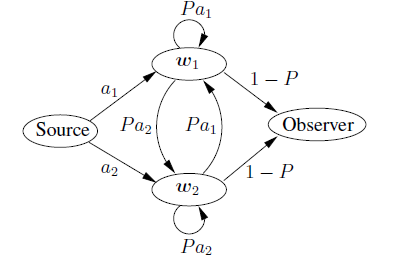
\includegraphics[width=0.4\textwidth]{multi.PNG}
\caption{Markov-ketting van het multilineair model \label{fig:multi}}
\end{wrapfigure}

De inkomende lichtstraal valt in op een materiaal binnen een pixel. Wanneer deze invalt op het materiaal heeft deze een kans $P$ om opnieuw in te vallen op hetzelfde of een ander materiaal in dezelfde pixel, en een kans $(1 - P)$ om te reflecteren naar de detector. De kans voor de gereflecteerde lichtstraal om in te vallen op een specifiek materiaal is gelijk aan diezelfde kans voor een lichtstraal afkomstig van de bron, namelijk de abundantie van de materiaal. Het spectrum van de lichtstraal verandert bij elke interactie zoals beschreven in sectie \ref{sec:ref}. Dat wil zeggen dat de uitgaande lichtstraal het elementwijs product is van de invallende lichtstraal en het albedo van het materiaal.
Dit hele proces kan worden voorgesteld als een Markov-ketting (zie figuur \ref{fig:multi}).

%\begin{enumerate}
%\item De inkomende straal interageert met minstens \'e\'en materiaal in de bron.
%\item Na deze interactie heeft het materiaal een kans $P$ om een nieuwe interactie aan te gaan, en een kans $(1-P)$ om dat niet te doen.
%\item De kans om een nieuwe interactie aan te gaan met elk nieuw materiaal is evenredig met de abundantie van dat materiaal. Merk op dat aangezien de som van de abundaties \'e\'en is, de waarde van de kans gelijk is aan de abundantie.
%\item Wanneer een lichtstraal interageert met een materiaal wordt zijn spectrum gewijzigd, afhankelijk van het albedo van dit materiaal.
%\end{enumerate}

\subsection{Berekening}

In deze sectie noemen we het "pad" van een lichtstraal de verzameling van de verschillende endmembers waarop het materiaal reflecteert, waarbij er rekening wordt gehouden met de volgorde. De kans dat een welbepaald pad gevolgd wordt, wordt als volgt genoteerd:

\begin{equation}
\mathcal{P}(i_1,i_2,i_3,...,i_R)
\end{equation}

Deze uitdrukking geeft de kans weer dat een lichtstraal reflecteert op materiaal $i_1$, daarna op $i_2$, op $i_3$ en zo voort, totdat deze uiteindelijk interageren met materiaal $i_R$. $R$ is hier het totaal aantal materialen waarop gereflecteerd wordt.

De kans op dit pad kan worden uitgerekend aan de hand van het hiervoor genoemde Markov-proces\cite{mlinmix}. 

\begin{equation}
\mathcal{P}(i_1,i_2,i_3,...,i_R) = P^{R-1} (1-P) \prod_{k=1}^R a_{i_k}
\end{equation}

Het spectrum van de uitgaande straal ten gevolge van een specifiek pad is $\Odot_{k=1}^R \bm{w}_{i_k}$, waarbij $\bm{w}_{i_k}$ het albedo is van materiaal $i_k$, en $\Odot$ het elementwijs product. Hiermee kan de bijdrage van een specifiek pad -de kans vermenigvuldigt met het spectrum- berekend worden als volgt:
\begin{equation}
\bm{x}_{(i_1,i_2,i_3,...,i_R)} = P^{R-1} (1-P) \Odot_{k=1}^R \left(a_{i_k} \bm{w}_{i_k}\right)
\end{equation}

Gesommeerd over alle mogelijke paden geeft dit het totale reconstructiespectrum. Deze som over alle paden kan berekend worden door de som te nemen over alle mogelijke waarden van $R$ voor een enkel pad, en dan als $R$ -het aantal interacties- gekend is, kan er voor elke interactie gesommeerd worden over alle materialen. Wanneer alle bijdragen van elk pad gesommeerd zijn over alle paden, geeft dit het totale spectrum dat de detector meet, en dit is gelijk aan:

\begin{equation}
\bm{x} = \sum_{R=1}^{\infty} \left(\sum_{i_1}^{p} ... \sum_{i_R}^{p}\right)P^{R-1} (1-P) \Odot_{k=1}^R \left(a_{i_k} \bm{w}_{i_k}\right)
\end{equation}

Stel dat de kans dat een lichtstraal nog een keer interageert, afhankelijk is van het materiaal, dan kan de kans dat een specifiek pad gevolgd word op analoge wijze worden berekend.

\begin{align}
\mathcal{P}(i_1,i_2,i_3,...,i_R) &= \prod_{k=1}^{R-1}P_{i_k} (1-P_{i_R})\\
&= \prod_{k=1}^{R}P_{i_k} \frac{1-P_{i_R}}{P_{i_R}}
\end{align}
Waarbij $P_{i_k}$ de reflectiekans van materiaal $i_k$ is. 

Het spectrum afkomstig van een specifiek pad wordt:

\begin{align}
\bm{x}_{(i_1,i_2,i_3,...,i_R)} &= \prod_{k=1}^{R-1}P_{i_k} (1-P_{i_R}) \Odot_{k=1}^R \left(a_{i_k} \bm{w}_{i_k}\right) \\
&= \Odot_{k=1}^{R-1} \left(P_{i_k}a_{i_k} \bm{w}_{i_k}\right) \odot (1-P_{i_R}) a_{i_R} \bm{w}_{i_R} \\
\bm{x} &= \sum_{R=1}^{\infty} \left(\sum_{i_1}^{p} ... \sum_{i_R}^{p}\right) \Odot_{k=1}^{R-1} \left(P_{i_k}a_{i_k} \bm{w}_{i_k}\right) \odot (1-P_{i_R}) a_{i_R} \bm{w}_{i_R} \\
&= \sum_{i=1}^p (1-P_i) a_{i} \bm{w}_{i} + \sum_{i=1}^p \sum_{j=1}^p (1-P_i) a_{i} \bm{w}_{i} \odot P_j a_{j} \bm{w}_{j} \nonumber\\&+ \sum_{i=1}^p \sum_{j=1}^p \sum_{k=1}^p (1-P_i) a_{i} \bm{w}_{i} \odot P_j a_{j} \bm{w}_{j} \odot P_k a_{k} \bm{w}_{k} \nonumber\\&+ \sum_{i=1}^p \sum_{j=1}^p \sum_{k=1}^p  \sum_{l=1}^p (1-P_i) a_{i} \bm{w}_{i} \odot P_j a_{j} \bm{w}_{j} \odot P_k a_{k} \bm{w}_{k} \odot P_l a_{l} \bm{w}_{l} \nonumber \\& + ... \\
&= \bm{z} + \bm{y}\odot\bm{z} + \bm{y}\odot\bm{y}\odot\bm{z} + ... \\
&= \bm{z} + \bm{y}\odot\bm{x} \\
 &= \frac{\bm{z}}{1-\bm{y}}
\end{align}
waar
\begin{align}
\bm{y} &= \sum_{i=1}^p P_i a_{i} \bm{w}_{i} \\
\bm{z} &= \sum_{i=1}^p (1-P_i) a_{i} \bm{w}_{i} 
\end{align}
zodat
\begin{equation}
\bm{x} = \frac{\sum_{i=1}^p (1-P_i) a_{i} \bm{w}_{i}}{1-\sum_{i=1}^p P_i a_{i} \bm{w}_{i}} \label{eq:Pi}
\end{equation}

Dit is een uitdrukking voor het multilineair mengen van endmembers waarbij de reflectiekans endmember-afhankelijk is. Indien men ge\"intereseerd is in een onafhankelijke reflectiekans, kan men de formule hiervoor bekomen door te stellen dat $P_i = P \forall i$ zodat het reconstructiespectrum gelijk wordt aan:

\begin{equation}
\bm{x} = \frac{(1-P) \sum_{i=1}^p a_{i} \bm{w}_{i}}{1-P\sum_{i=1}^p  a_{i} \bm{w}_{i}} \label{eq:P}
\end{equation}

wat exact overeenkomt met de formule in de literatuur\cite{mlinmix}.

Om aan de hand van dit model te ontmengen, moet nog steeds gebruik gemaakt worden van het minimaliseren van de reconstructie-error. 

\begin{align}
\text{argmin}_{a_1 ... a_p; P_1 ... P_p} \left| \bm{x} - \frac{\sum_{i=1}^p (1-P_i) a_{i} \bm{w}_{i}}{1-\sum_{i=1}^p P_i a_{i} \bm{w}_{i}} \right|^2
\end{align}

Aangezien deze vergelijking niet lineair is en bijgevolg ook geen hypervlak opspant, kan deze uitdrukking niet geminimaliseerd worden door middel van projecties, en zijn er hier geavanceerde minimalisatietechnieken nodig. In matlab\cite{MATLAB} wordt voor deze thesis hiervoor de functie \texttt{fmincon} gebruikt. Deze neemt de uitdrukking $\left| \bm{x} - \frac{\sum_{i=1}^p (1-P_i) a_{i} \bm{w}_{i}}{1-\sum_{i=1}^p P_i a_{i} \bm{w}_{i}} \right|^2$ in en geeft hier een minimum voor terug. Dit heeft als nadeel dat het draaien van deze functie op de experimentele data later beschreven in deze thesis, een looptijd heeft van ongeveer $0.1$ seconden per pixel, in tegenstelling tot het berekenen van pseudo-inversen, wat ongeveer $50$ microseconden in beslag neemt. 

\subsection{Reflectantie vs albedo}

Het albedo $\bm{w}_i$ uit vorige sectie kan niet exact gemeten worden. In theorie kan deze afgeleid worden uit de reflectie van een meting met een enkele endmember. Dit kan bepaald worden door vergelijking \ref{eq:Pi} te inverteren, zodat:

\begin{equation}
\bm{w}_i = \frac{\bm{e}_i}{\bm{e}_iP_i + 1 - P_i}
\end{equation}
waarbij de deling de elementwijze deling is. 

Hierbij wordt verondersteld dat $P_i$ gekend is, wat in werkelijkheid niet het geval is. Daarom wordt verondersteld dat $P_i \approx 0$ wat neerkomt op een benadering die stelt dat $\bm{w}_i \approx \bm{e}_i$. 

\subsection{Ondergrens van P waarde}

$P$ is per definitie een getal groter dan nul, omdat kansen tussen nul en \'e\'en liggen. Echter, het is mogelijk om in vergelijking \ref{eq:Pi} een negatieve waarde in te voeren. Deze waarde kan negatief zijn in twee situaties. Enerzijds - zoals beschreven in de vorige sectie- is het albedo slechts een benadering. Doordat de reflectie van de referentie-endmember nul wordt verondersteld te zijn, is deze lager dan in werkelijkheid. Bijgevolg zal ook de reflectiekans van de pixel lager zijn dan in werkelijkheid. In het geval dat de reflectiekans van de pixel lager is dan de reflectiekans van het referentiemateriaal, ligt deze waarde onder nul. Merk op dat dit systeem niet lineair is, waardoor een verkeerde reflectiekans in bovengenoemde sectie niet kan opgelost worden door het herdefini\"eren van $P$. Anderzijds, zijn er ook interpixel-interacties die invloed hebben op het systeem. Deze kunnen extra lichtstralen die hebben gereflecteerd op een materiaal in een andere pixel toevoegen aan het systeem, wat zorgt voor een verlaging van de reflectiekans. 

%\subsection{afhankelijke vs onafhankelijke P waarden}





\section{multiple endmember spectra mixture analysis} \label{sec:mesma}

Om te ontmengen rekening houdend met variabiliteit is elke endmember een bibliotheek van verschillende spectra. Het extraheren van deze spectra uit de metingen ligt buiten het bestek van deze thesis, hier wordt gewoon vanuitgegaan dat de endmembers gekend zijn. De experimentele data beschouwd in deze thesis bevat spectra die vanop de grond gemeten worden aan de hand van een spectrograaf, en zijn dus exact gekend.

Het \textit{multiple endmember spectra mixture analysis} ofwel \textit{MESMA} algoritme gaat ervan uit dat elk materiaal in elke pixel maar een enkel spectrum reflecteert, maar dit spectrum kan verschillen tussen verschillende pixels.  Merk op dat materialen die zich niet bevinden in een pixel ook geen toegewezen spectrum hebben. Deze spectra en de abundanties van de respectievelijke materialen worden gevonden door te ontmengen in functie van alle mogelijke spectra voor alle mogelijke deelverzamelingen van materialen, en daarna wordt de ontmenging geselecteerd met de laagste reconstructie-error. De volgende secties leggen deze procedure uit in meer detail.

\subsection{deelverzameling van alle materialen}

Als eerste moet er gelopen worden over alle mogelijke deelverzameling van materialen. Voor elke deelverzameling geldt dat een enkel materiaal daar ofwel een element van is, ofwel niet. Hierdoor zijn er $2^p$ mogelijke deelverzamelingen. Er kan ge\"itereerd worden over alle deelverzamelingen door te itereren over de natuurlijke getallen van nul tot $2^p-1$. Elke waarde van deze iterator kan geschreven worden als een binair getal, waarbij elk cijfer daarvan bepaald of het materiaal vervat zit in de deelverzameling of niet. De waarde nul is de lege deelverzameling, dus deze wordt overgeslagen, en de iterator begint bij een.

\subsection{Itereren over alle bibliotheken}

Wanneer beslist is welke materialen een pixel bevat, moet ge\"iterereerd worden over alle mogelijke spectrum van elk materiaal. Er zijn verschillende methoden om te intereren over verschillende verzamelingen, zoals bijvoorbeeld de \textit{Banker series}, maar in deze thesis wordt gebruik gemaakt van de overvloedige tellers. Dit houdt in dat men een vector gebruikt als index, waarbij elk element verwijst naar een enkel materiaal, en de waarde van dit element verwijst naar de index van het spectrum dat gekozen wordt voor dit materiaal. Elke lus wordt de vector gewijzigd zoals weergegeven in \ref{al:oc}.

\begin{algorithm}
\caption{Overvloedige tellers\label{al:oc}}
\begin{algorithmic}[1]
\State de vector begint met overal 1
\While {True}
\State verhoog het eerste element met 1
\For {voor elk element}
\If {Indien het element hoger is dan zijn maximum (het aantal spectra voor het respectievelijke materiaal)}
\State zet het element op 1
\State verhoog het volgende element met 1
\State indien dit element het laatste element is, be\"eindig het algoritme.
\EndIf
\EndFor
\EndWhile
\end{algorithmic}
\end{algorithm}

\subsubsection{Voorbeeld van overvloedige tellers}

Stel dat er gebruik gemaakt wordt van de voorgenoemde \textit{Alina dataset}. Deze bevat vier materialen, namelijk bebossing, asfalt, de stoeprand en gras. Deze vier materialen hebben elk een bibliotheek van respectievelijk 50, 10, 10 en 10 materialen. Beschouw nu een pixel waarvan bekend is dat deze uit bos, asfalt en gras bestaat. Dan evolueerd de indexvector als volgt:

\begin{itemize}
\item De vector begint met waarde $[1,1,1]$.
\item Na de eerste stap wordt de waarde van deze vector $[2,1,1]$.
\item Het eerste element blijft elke stap toenemen tot het de waarde 50 bereikt. De vector is nu gelijk aan $[50,1,1]$.
\item De volgende stap wordt deze waarde $[1,2,1]$.
\item Hierna neemt het eerste element weer toe, tot dat dit terug de waarde 50 bereikt. De vector is nu gelijk aan $[50,2,1]$.
\item Zoals voordien blijft dit lopen tot de vector de waarde $[50,10,1]$ bereikt.
\item De volgende stap wordt het eerste element op 1 gezet moet het tweede element verhogen, maar omdat dit element ook groter wordt dan het maximum, wordt dit ook op een gezet en wordt het laatste element verhoogt. Dit resulteert in een vector gelijk aan $[1,1,2]$.
\item Dit proces wordt verder herhaald tot de vector gelijk is aan $[50,10,10]$. Hierna overstroomt het laatste element en eindigt het algoritme. 
\end{itemize}

Na deze procedure zijn alle 5000 mogelijke waarde dat de indexvector kan aannemen afgegaan.

\subsection{Ontmengen van de selectie}

In de vorige secties zijn de materialen en de correcte spectra geselecteerd. Hierna kan de pixel worden ontmengd zoals in vorig hoofdstuk, gebruikt makend van het \textit{sum-to-one constrained least-squares unmixing model}. Dit model houdt geen rekening met de niet-negativiteitsvoorwaarde, en kan bijgevolg negatieve abundaties bekomen. Indien dit gebeurt, wordt deze selectie overgeslagen, en wordt overgegaan naar de volgende selectie van spectra en materialen. Dit is een logische keuze, aangezien indien een materiaal optimaal een negatieve hoeveelheid heeft, er beter kan worden overgegaan op een ander systeem, dat dit materiaal niet bevat. Merk op dat het onmogelijk is dat alle selecties worden verwijderd aan de hand van deze voorwaarde, aangezien dat de deelverzamelingen met een enkel materiaal dit materiaal dankzij de eenheidssom-voorwaarde een abundantie van $1$ heeft. Het hele proces wordt beschreven in algoritme \ref{al:mesma}.

\begin{algorithm}
\caption{MESMA\label{al:mesma}}
\begin{algorithmic}[1]
\State $\eta = +\infty$ 
\For {Voor alle deelverzamelingen}
\For {Voor alle combinaties van spectra}
\State Ontmeng gebruik makend van het \textit{sum-to-one constrained least-squares unmixing model}
\If {$\exists \text{Abundantie} < 0$}
\State \textbf{continue}
\EndIf
\If {reconstructie-error $< \eta$}
\State $\eta = $ reconstructie-error
\State $a_i = $ abundanties
\EndIf
\EndFor
\EndFor
\State $a_i$ zijn nu de correcte abundanties
\end{algorithmic}
\end{algorithm}

\subsection{vrije keuze van het ontmeng-algoritme}
Hierboven is gebruikt gemaakt van het lineaire ontmeng algoritme, maar dit hoeft niet het geval te zijn. In algoritme \ref{al:mesma} kan de regel \texttt{Ontmeng gebruik makend van het \textit{sum-to-one constrained least-squares unmixing model}} vervangen worden door elk algoritme naar keuze. Indien men ge\"intereseert is in niet lineaire effecten, kan hier gebruik gemaakt worden van het multilineair model. Echter, voor de Alina dataset gebruikt in deze thesis, die alleen al voor de deelverzameling van alle materialen $50\times 10\times 10 \times 10= 50000$ mogelijkheden bevat, en waarvoor het ontmengen van een pixel aan de hand van vier spectra ongeveer $0.1$ seconden duurt, neemt dit algoritme meer dan $2 uur$ in beslag voor elke pixel. Het beeld bevat ongeveer de 400 pixels, dus de totale looptijd van dit algoritme is ongeveer $25 dagen$. 

\section{Hoekminimalisatie}

Het lineair ontmengen gebeurd door het gemeten spectrum te projecteren op het hypervlak opgespannen door de endmembers. Noemen we dit hypervlak $S$, den kan de reconstructie-error herschreven worden als:

\begin{equation}
\left| \bm{x} - \proj{\bm{x}}{S}\right|
\end{equation}

Noemen we $F$ het hypervlak opgespannen door endmembers $\left\{ e_1 , ... e_{p-1} \right\}$, zijnde het hypervlak opgespannen door alle endmembers behalve $e_p$ dan geldt:

\begin{equation}
\left| \bm{x} - \proj{\bm{x}}{S}\right|  = \left| \bm{x} - \proj{\bm{x}}{F}\right| \sin \theta
\end{equation}

Met 

\begin{align}
\theta &= \min(\alpha, \pi-\alpha) \\
\alpha &= \arcsin \left(\frac{\left|x - \proj{x}{S}\right|}{\left|x - \proj{x}{F}\right|}\right)
\end{align}

In deze laatste uitdrukking kan de rol van $e_p$ en $x$ worden verwisseld, dus als er gesteld wordt dat $G$ het hypervlak opgespannen door $\left\{ e_1 , ... ,e_{p-1}, x \right\}$ is, geldt dat:

\begin{equation}
\alpha = \arcsin \left(\frac{\left|e_p - \proj{e_p}{G}\right|}{\left|e_p - \proj{e_p}{F}\right|}\right)
\end{equation} 

Aangezien in functie van $e_p$, $\left| \bm{x} - \proj{\bm{x}}{F}\right|$ constant is, zal de minimalisatie van $\sin \theta$ de reconstructie-error minimaliseren. De optimale hoek kan gevonden worden door deze uit te rekenen voor elk bibliotheekelement en het minimum uit te kiezen.

\subsection{optimalistatie}

Om deze techniek toe te passen voor de selectie van spectra voor de endmembers, kan een optimalisatieprocesdure gebruikt worden. Men begint met een willekeurige selectie van bibliotheekelementen. Daarna wordt voor een elk materiaal het optimale spectrum bepaald, terwijl de andere materialen constant gehouden worden. Dit wordt herhaalt, totdat er voor geen enkel materiaal nog een verbetering van de spectrale hoek bestaat. Aangezien er een eindig aantal mogelijkheden zijn voor de keuze van spectra en dat de reconstructie-error kleiner wordt bij elke stap, eindigt dit algoritme met zekerheid. In praktijk wordt echter vaak een maximum aantal iteraties gebruikt, omdat dit computationeel eenvoudiger is. Het volledige proces staat beschreven in \ref{al:AAM}

\begin{algorithm}
\caption{\textit{Alternating Angle Minimalistation} \label{al:AAM}}
\begin{algorithmic}[1]
\State kies een aantal iteraties $K$
\For {Voor elke deelverzameling van materialen}
\State Stel $q$ het aantal materialen
\State Stel $e_j^i$ het $j$-de spectrum uit de bibliotheek van het $i$-de materiaal.
\State Selecteer een willekeurige index set $I_j$
\For {doe $K$ keer} 
\For {voor $i$ elk materiaal}
\State Definieer F het hypervlak opgespannen door $\{e^1_{I_1},...,e^{i-1}_{I_{i-1}},e^{i+1}_{I_{i+1}},...,e^q_{I_q}\}$
\State Defineer G het hypervlak opgespannen door bovenstaande endmembers en $\bm{x}$
\For {n $\in [1,...,\text{aantal spectra}]$}
\State $p_n = \arcsin \left(\frac{\left|e^i_n - \proj{e^i_n}{G}\right|}{\left|e^i_n - \proj{e^i_n}{F}\right|}\right)$
\If {$(e^i_n - \proj{e^i_n}{F}) \dot (x - proj{x}{F}) < 0$}
\State $p_n = \pi - p_n$
\EndIf
\EndFor
\EndFor
\State $I_n = \text{argmin}_n\left(p_n\right)$
\EndFor
\State $E = [e_{I_1},...,e_{I_p}]$
\State Abundantie en reconstructie-error kan bepaald worden aan de hand van het \textit{Fully constrained
least-squares unmixing model} met als endmembers $E$
\EndFor
\State geef het resultaat terug uit vorige stap met de laagste reconstructie-error.
\end{algorithmic}
\end{algorithm}


\chapter{Variabiliteit voor niet-lineaire systemen.}

\section{Semi-lineair model}

ontkoppeling van Ontmenging in MESMA bij selectie tov ontmenging voor abundancies

\subsection{Theoretische controle dmv monte carlo simulaties}

\section{multilineair AAM}

\chapter{experimentele vergelijking van verschillende methodes}

\section{looptijd en reconstructie-error}

\section{Alina dataset}

\section{Lijst en korte uitleg bij alle methodes}

Elke methode is hiervoor beschreven, maar dit beschrijft kort de verschillen in de methodes en hoe deze ge\"implementeerd zijn door middel van `schakelaars' in de code. Ook een uitleg bij de weergave van de resultaten. 

\begin{itemize}
\item lineair MESMA
\item semi-lineair MESMA
\item multi-lineair MESMA
\item lineair AAM
\item multilineair AAM
\end{itemize}

$\rightarrow$ Voor de multilineaire modellen wordt ook al dan niet $P> 0$ en $P$ materiaalafhankelijk vergeleken.



\section{Bepreking lineair vs semi-linair}

Verschil voor hoge reflectie (bomen)
$\rightarrow$ semilineair geeft betere resultaten voor dezelfde runtime

\section{Bespreking semi-lineair vs multilineair}

$\rightarrow$ semilineair geeft vergelijkbare resultaten op kortere tijd

\section{Bespreking P-afhankelijkheid}

$\rightarrow$ P-afhankelijkheid geeft vergelijkbare resultaten op gelijke tijd, maar heeft meer vrijheidsgraden

\section{Bespreking P-ondergrens}

verschil voor lage reflectie (asfalt)
$\rightarrow$ Weglaten van ondergrens geeft betere resultaten op gelijke tijd.

\section{Bepreking multilinair AAM vs semilinair model}

$\rightarrow$ zelfde resultaten voor kortere tijd.

\begin{appendices}


\end{appendices}


\begin{flushleft}
\nocite{*}
\bibliography{biblio}{}
\bibliographystyle{plain}
\addcontentsline{toc}{chapter}{Bibliografie}

\end{flushleft}


\end{document}
